\documentclass[11pt]{article}
\usepackage[a4paper,margin=2.3cm]{geometry}
\usepackage{amsmath,amssymb}
\usepackage{booktabs}
\usepackage{tikz}
\usetikzlibrary{positioning,arrows.meta,calc}
\usepackage[hidelinks]{hyperref}
\usepackage{parskip}
\usepackage{enumitem}
\setlist{itemsep=2pt,topsep=2pt}

\newcommand{\x}{\mathbf{x}}
\newcommand{\z}{\mathbf{z}}
\newcommand{\m}{\mathbf{m}}
\newcommand{\T}{^{\top}}

\title{\textbf{The group lasso in EXTRACT}\\[2pt]\large what is fitted, how, and how it enters training (branch \texttt{main})}
\author{EXTRACT project notes}
\date{\today}

\begin{document}
\maketitle

\section{The idea in one paragraph}

Every row of the data is the response of one (perturbation, context) pair: the
pair's full-data estimate or one of its 100-cell pseudobulks. We write each row
as a combination of the $d=20$ programs, $\x \approx \z B$. Without sparsity, a
row may use all 20 programs. The group lasso asks for the opposite: each
\emph{pair} should use only a few programs, and all rows of the same pair must
use the \emph{same} few. How strongly each chosen program is used may still
differ between the rows of the pair. A perturbation can use different programs
in different contexts, because each (perturbation, context) pair makes its own
choice.

\section{What is fitted}

\paragraph{Notation.}
\begin{itemize}
  \item $B$: the $d\times G$ loadings, one row $\mathbf b_k$ per program
  ($G=5{,}504$ genes, no mitochondrial genes). In the fixed mode $B=AV$, with
  $V$ the PCA of the training pair means (fixed) and $A$ learned. Every row of
  $B$ is kept at unit length.
  \item A pair $g$ has $n_g$ rows $\x_1,\dots,\x_{n_g}$ (full row + pseudobulks;
  all rows of a pair are exchangeable, the model is not told which is which or
  how many cells they have).
  \item $Z_g$: the $n_g\times d$ activities of the pair's rows; row $r$ is
  $\z_r$, column $k$, written $Z_g[:,k]$, is program $k$'s activity in each of
  the pair's rows.
  \item $\m_r$: a 0/1 mask over genes that removes the row's own target gene
  (its knockdown would dominate).
\end{itemize}

\paragraph{The objective, for one pair.}
\begin{equation}
  \min_{Z_g}\;\;
  \underbrace{\tfrac12\sum_{r=1}^{n_g}\big\|\m_r\odot(\x_r-\z_r B)\big\|^2}_{\text{reconstruction error}}
  \;+\;
  \underbrace{\lambda\,\sqrt{n_g}\,\sum_{k=1}^{d}\big\|Z_g[:,k]\big\|_2}_{\text{group penalty}}
  \label{eq:gl}
\end{equation}

\begin{itemize}
  \item \textbf{The penalty acts on columns.} $\|Z_g[:,k]\|_2$ is the length of
  program $k$'s activity vector across the pair's rows. A group penalty on such
  lengths sets whole columns exactly to zero: program $k$ is then off for
  \emph{every} row of the pair. A column that survives can take any values, so
  the rows of the pair may use a chosen program with different strengths.
  \item \textbf{$\sqrt{n_g}$} makes the penalty comparable between pairs with
  few and many rows (a column's length grows like $\sqrt{n_g}$).
  \item \textbf{$\lambda$} sets how few programs a pair uses: larger $\lambda$,
  fewer programs.
  \item \textbf{Unit-length rows of $B$ are required.} Otherwise a program could
  be scaled up, its activities scaled down by the same factor, and the penalty
  would shrink for free.
\end{itemize}

\begin{figure}[h]
\centering
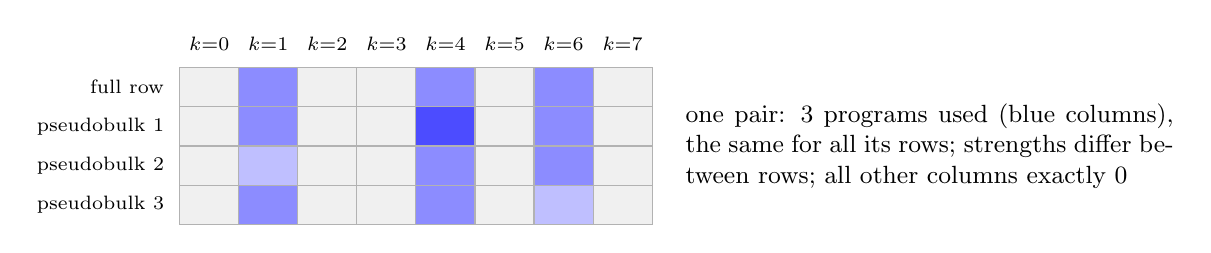
\begin{tikzpicture}[x=0.75cm,y=0.5cm]
  \foreach \c in {0,...,7} \foreach \r in {0,...,3}
    \fill[gray!12] (\c,-\r) rectangle ++(1,-1);
  \foreach \c in {1,4,6} \foreach \r in {0,...,3}
    \fill[blue!45] (\c,-\r) rectangle ++(1,-1);
  \fill[blue!25] (1,-2) rectangle ++(1,-1); \fill[blue!70] (4,-1) rectangle ++(1,-1); \fill[blue!25] (6,-3) rectangle ++(1,-1);
  \draw[step=1,gray!60] (0,0) grid (8,-4);
  \foreach \c in {0,...,7} \node[font=\scriptsize] at (\c+0.5,0.6) {$k{=}\c$};
  \node[font=\scriptsize,anchor=east] at (-0.1,-0.5) {full row};
  \foreach \r in {1,2,3} \node[font=\scriptsize,anchor=east] at (-0.1,-\r-0.5) {pseudobulk \r};
  \node[font=\small,anchor=west] at (8.4,-2) {\parbox{6.2cm}{one pair: 3 programs used (blue columns),
  the same for all its rows; strengths differ between rows; all other columns exactly 0}};
\end{tikzpicture}
\caption{What the group lasso produces for one pair (8 of the 20 programs shown).}
\end{figure}

\section{How it is solved}

Equation~\eqref{eq:gl} has no closed form; it is solved by
\textbf{FISTA} (proximal gradient with momentum), separately for every pair,
all pairs of a batch in parallel:
\begin{enumerate}
  \item \textbf{Start} at the least-squares activities (the masked projection of
  each row onto $B$).
  \item \textbf{Gradient step} on the reconstruction error, step size
  $\eta=1/L$ with $L$ the largest eigenvalue of $BB\T$.
  \item \textbf{Group soft-thresholding} of each column:
  \[
    Z_g[:,k]\;\leftarrow\;Z_g[:,k]\cdot\max\!\Big(0,\;1-\frac{\eta\,\lambda\sqrt{n_g}}{\|Z_g[:,k]\|_2}\Big),
  \]
  which shrinks every column and sets the small ones exactly to zero.
  \item \textbf{Momentum} (the FISTA extrapolation), and repeat; 30 steps.
\end{enumerate}
The programs whose column is non-zero at the end are the pair's \textbf{selected
programs}. On the real data, 30 steps select the same programs as 150 steps in
99.7--99.9\% of cases. The steps are ordinary differentiable operations, so
gradients flow back to $B$ through them (the starting point is held fixed).

\paragraph{One fit.} The same activities are used everywhere: in the
reconstruction objective below and by the discriminator.

\section{How it enters training}

\paragraph{Loss.} With the group lasso and only label swaps as false examples
(the chosen setting; no shuffled rows), the training loss is
\begin{equation}
  \text{total} \;=\; L_\text{disc} \;+\; \alpha\,L_\text{lasso},
  \qquad
  L_\text{lasso} \;=\; \frac1{n}\sum_{\text{rows}} \frac{\|\m_r\odot(\x_r-\z_r B)\|^2}{G}
  \;+\; \frac{2\lambda}{nG}\sum_{\text{pairs } g}\sqrt{n_g}\sum_k\|Z_g[:,k]\|_2 ,
\end{equation}
with $n$ the number of rows in the batch and $Z$ the lasso activities. $L_\text{lasso}$ is exactly equation~\eqref{eq:gl}, summed over the
batch's pairs and divided by $nG/2$, so it is on the same per-row, per-gene
scale as before. $L_\text{disc}$ is the binary discriminator loss on the same
activities ($\alpha=700$).

\paragraph{$\lambda$ appears twice.} In the solve (which programs each pair
selects) and in the loss (so the gradient on $A$ feels the penalty: axes on which
pairs need fewer programs become cheaper).

\paragraph{Per step.}
\begin{enumerate}
  \item A batch is made of \emph{whole pairs} (all rows of a pair together),
  about 1{,}024 rows.
  \item Solve equation~\eqref{eq:gl} for every pair of the batch with the
  current $B$.
  \item Compute $L_\text{disc}$ and $L_\text{lasso}$ on these activities;
  backpropagate; one optimiser step on $A$ and the label network.
  \item Rescale the rows of $B=AV$ to unit length.
\end{enumerate}
Validation and inference also need whole pairs: each row must be solved
together with the other rows of its pair.

\section{Choosing $\lambda$}

The natural scale of $\lambda$ is the typical size of a program's activity in a
pair. We measured it as the median, over pairs and programs, of
$\|Z_g[:,k]\|_2/\sqrt{n_g}$ for the least-squares activities on the joint
diagonalisation axes: \textbf{0.0272} at $d=20$. The grid was
$\lambda\in\{1,2,4,7.4,14.7\}\times 0.0272$.

\begin{table}[h]
\centering\small
\begin{tabular}{lccccc}
\toprule
$\lambda$ & 0.0272 & 0.0544 & 0.1088 & 0.2 & 0.4 \\
\midrule
programs per pair (validation) & 6.2 & 3.9 & 2.2 & 1.3 & 0.6 \\
validation AUC & 0.808 & 0.763 & 0.726 & 0.686 & 0.645 \\
reconstruction explained & 51.7\% & 51.5\% & 51.2\% & 50.6\% & 49.4\% \\
\bottomrule
\end{tabular}
\caption{Chosen setting (4-statistics head with normaliser, label swaps only, JD
start, no-MT data), mean over 3 seeds. Fewer programs per pair cost
discrimination but barely any reconstruction: a pair's response is carried by
very few directions.}
\end{table}

\section{Why it helps choose the axes}

Reconstruction alone cannot choose the axes inside $V$: in the fixed mode every
rotation of the axes fits the data equally well. The group penalty can. If
the true programs are the axes, a pair's response lies on a few of them and
needs few non-zero columns. Rotate the axes, and the same response is spread
over many programs: more non-zero columns, a larger penalty. So the lasso
objective prefers axes on which pairs are sparse.

We checked this without any training, on 3{,}000 training pairs
($d=20$, $\lambda = 2\times$ scale, data with mitochondrial genes):

\begin{table}[h]
\centering\small
\begin{tabular}{lccc}
\toprule
axes & lasso objective & error & programs per pair \\
\midrule
ICA                         & 1.5267 & 1.4876 & 2.77 \\
PCA ($V$ itself)            & 1.5296 & 1.4848 & 2.27 \\
joint diagonalisation (JD)  & 1.5305 & 1.4884 & 2.83 \\
JD rotated, $t=0.25$        & 1.5312 & 1.4885 & 2.89 \\
JD rotated, $t=0.5$         & 1.5326 & 1.4887 & 2.94 \\
JD rotated, $t=1$           & 1.5357 & 1.4891 & 3.08 \\
JD rotated, $t=2$           & 1.5399 & 1.4895 & 3.18 \\
\bottomrule
\end{tabular}
\caption{The objective rises steadily as the axes are rotated away from JD,
mostly through the penalty (more programs per pair). The preference is real
but small, which is why, in training, the discriminator can still move the
axes.}
\end{table}

\section{What it does not do}

\begin{itemize}
  \item It does not make the \emph{gene} loadings sparse; it makes each pair
  use few programs. Sparsity over genes is a separate prior on $B$ (under
  discussion).
  \item It does not use labels, cell counts or the identity of the full row:
  the grouping only says which rows belong to the same pair.
  \item It does not force a perturbation to use the same programs in every
  context.
\end{itemize}

\end{document}
